
\subsection{Variation from the Original Algorithm}
To extend the shell formulation in~\ref{chp:shell} to accommodate for feature preservation (Section \ref{cumin:sec:features-pres}), we modify the definition of a valid section~\ref[Definition 3.1]{chp:shell}, by relaxing the intersection between a triangle and a prism in the discrete case. That is, we do not consider the prism to be intersecting a triangle if they share only one vertex of the triangle; we also ignore the intersection if they intersect on a feature edge on opposite sides. The bijectivity and validity condition of the shell projection trivially holds.

%%%%%%%%%%%%%%%%%%%%%%%%%%%%%%%%%%%%%%%%%%%
%%%%%%%%%%%%%%%%%%%%%%%%%%%%%%%%%%%%%%%%%%%

\begin{figure}
    \centering
    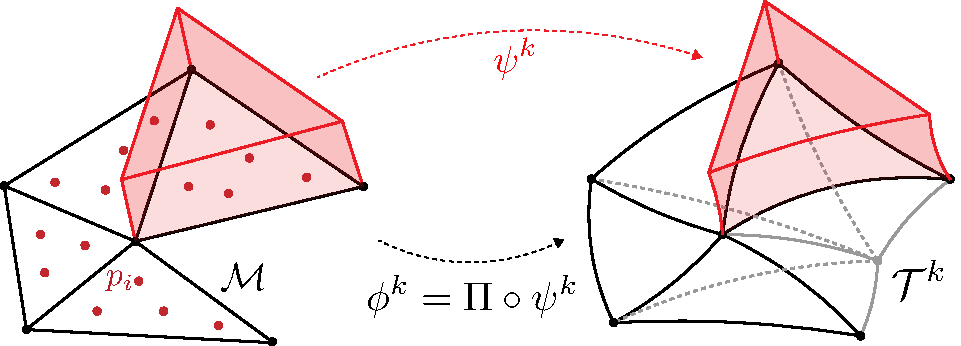
\includegraphics[width=.8\linewidth]{curve_meshing_in_shell_tex/figs/illustrations/input-output.pdf}
    \caption{Input triangle mesh $\M$ and points $\P$. Output curved tetrahedral mesh $\T^k$ and bijective map $\phi^k$.}
    \label{bichon:fig:input-output}
\end{figure}

\section{Curved Tetrahedral Mesh Generation}\label{cumin:sec:curved-pipeline}



\paragraph{Input.}
The input of our algorithm is a collection of oriented manifold, watertight, self-intersection-free triangle mesh $\M=(V,F)$, and a set of points $p_i\in\P$ (possibly empty) on the surface of $\M$ (Figure~\ref{bichon:fig:input-output}, left) where the distance bound $\varepsilon$ is prescribed. The collection $\M$ must be consistently oriented such that it is the boundary of an oriented 3-manifold.
A set of edges can also be optionally provided as annotated features (Section~\ref{cumin:sec:features-pres}).

\begin{figure}
    \centering
    % \includegraphics[width=.6\linewidth]{curve_meshing_in_shell_tex/figs/nodes}\hfill
    % \includegraphics[width=.37\linewidth]{curve_meshing_in_shell_tex/figs/gmapping}
    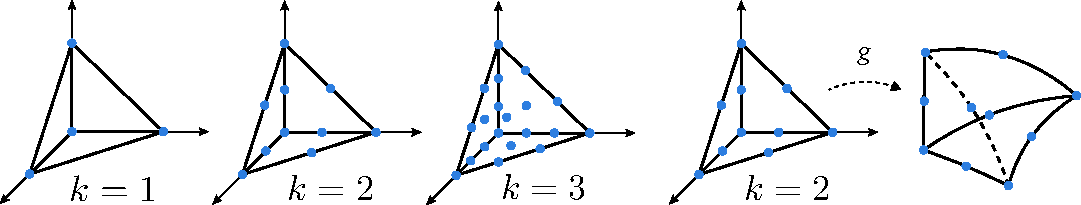
\includegraphics[width=\linewidth]{curve_meshing_in_shell_tex/figs/illustrations/high-order.pdf}
    \caption{Lagrange nodes on the reference element $\hat \tau$ for different $k=1,2,3$ and example of geometric mapping $g$.}
    \label{bichon:fig:high-order}
\end{figure}

\paragraph{Output.}
The output of our algorithm is a tetrahedral mesh $\T^k = (V^k,T^k)$ of order $k$. 
Formally, each tetrahedron $\tau\in T^k$ is defined through the \emph{geometric map} from the reference tetrahedron $\hat \tau$,
\begin{equation}\label{eq:gmap}
g^\tau = \sum_{j=1}^n c_j^\tau L_j(\hat u,\hat v,\hat w),
\end{equation}
where $\hat u,\hat v,\hat w$ are the local coordinates of a point in $\hat \tau$, $c_j^\tau$ are the control points for a tetrahedron $\tau$, and $L_j$ are polynomial bases (typically Lagrange bases).
For two tetrahedra $\tau_1$ and $\tau_2$ 
of $T^k$ sharing a face $F$, the restriction of the maps $g^{\tau_i}$, $i=1,2$, to $F$ coincide.
Figure~\ref{bichon:fig:high-order} shows the position of the control points $c_j$ on the reference element for $k=1,2,3$ for the Lagrange bases. We call the tetrahedralization of a curved mesh $\T^k$ \emph{positive} if $\det(J_{g^\tau}) > 0$ everywhere on every $\tau$. 
% That is, we require that the geometric mapping $g^T$ is bijective for every tetrahedron \DP{I don't think this is true, the implication holds the other way, discuss.} \DZ{Indeed this is obviously not true except in the linear case; positive Jacobian only guarantees local injectivity; a sufficient condition is that the map is bijective on the boundary}. 
In particular, for $k=1$, since $g$ is affine, $J_{g^\tau}$ is constant and the positivity reduces to the positive orientation of the vertices \cite{shewchuk1997adaptive}.

Note that, while bijectivity of the geometric map $g^\tau$ implies positivity, the reverse is not true. 
Therefore, our algorithm not only checks for $\det(J_{g^\tau}) > 0$, but also ensures that the boundary $\partial\T^k$ does not intersect; we show in Appendix~\ref{cumin:sec:bij-proof} that these two conditions guarantee the bijectivity of $g^\tau$.
Furthermore, our algorithm ensures that the distance from any point in $\P$ to $\partial\T^k$ (the surface of $\T^k$) is smaller than an user-controlled parameter $\varepsilon$.

\begin{figure}
    \centering\small
    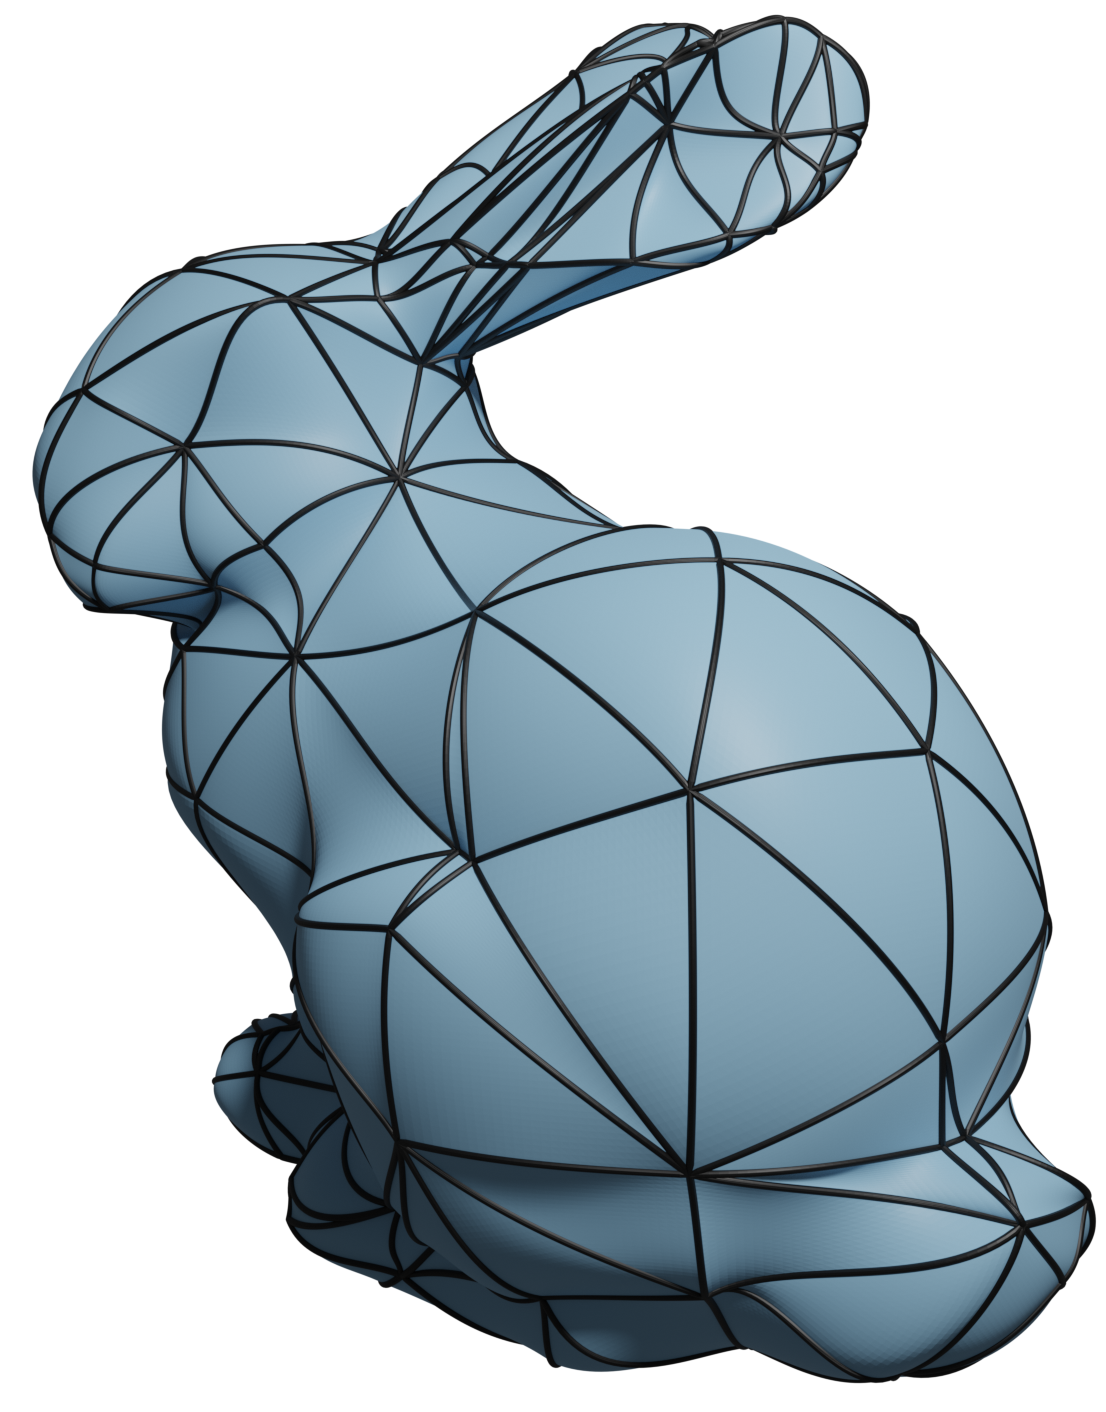
\includegraphics[width=0.23\linewidth]{curve_meshing_in_shell_tex/figs/bunny/0001}\hfill
    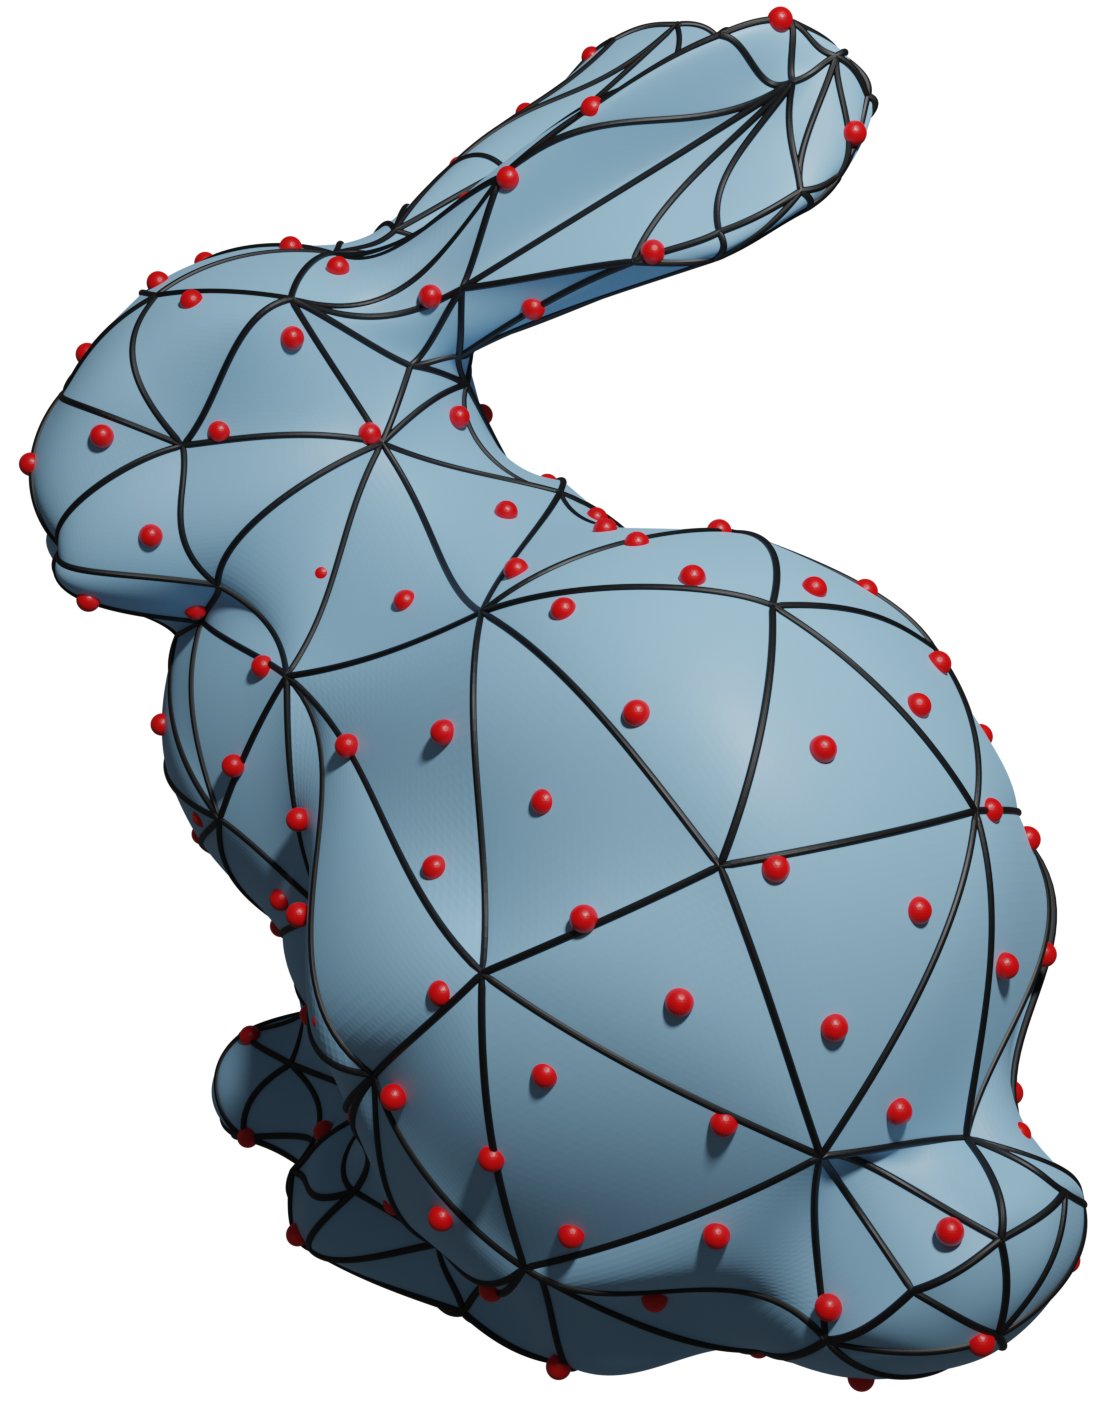
\includegraphics[width=0.23\linewidth]{curve_meshing_in_shell_tex/figs/bunny/0004}\hfill
    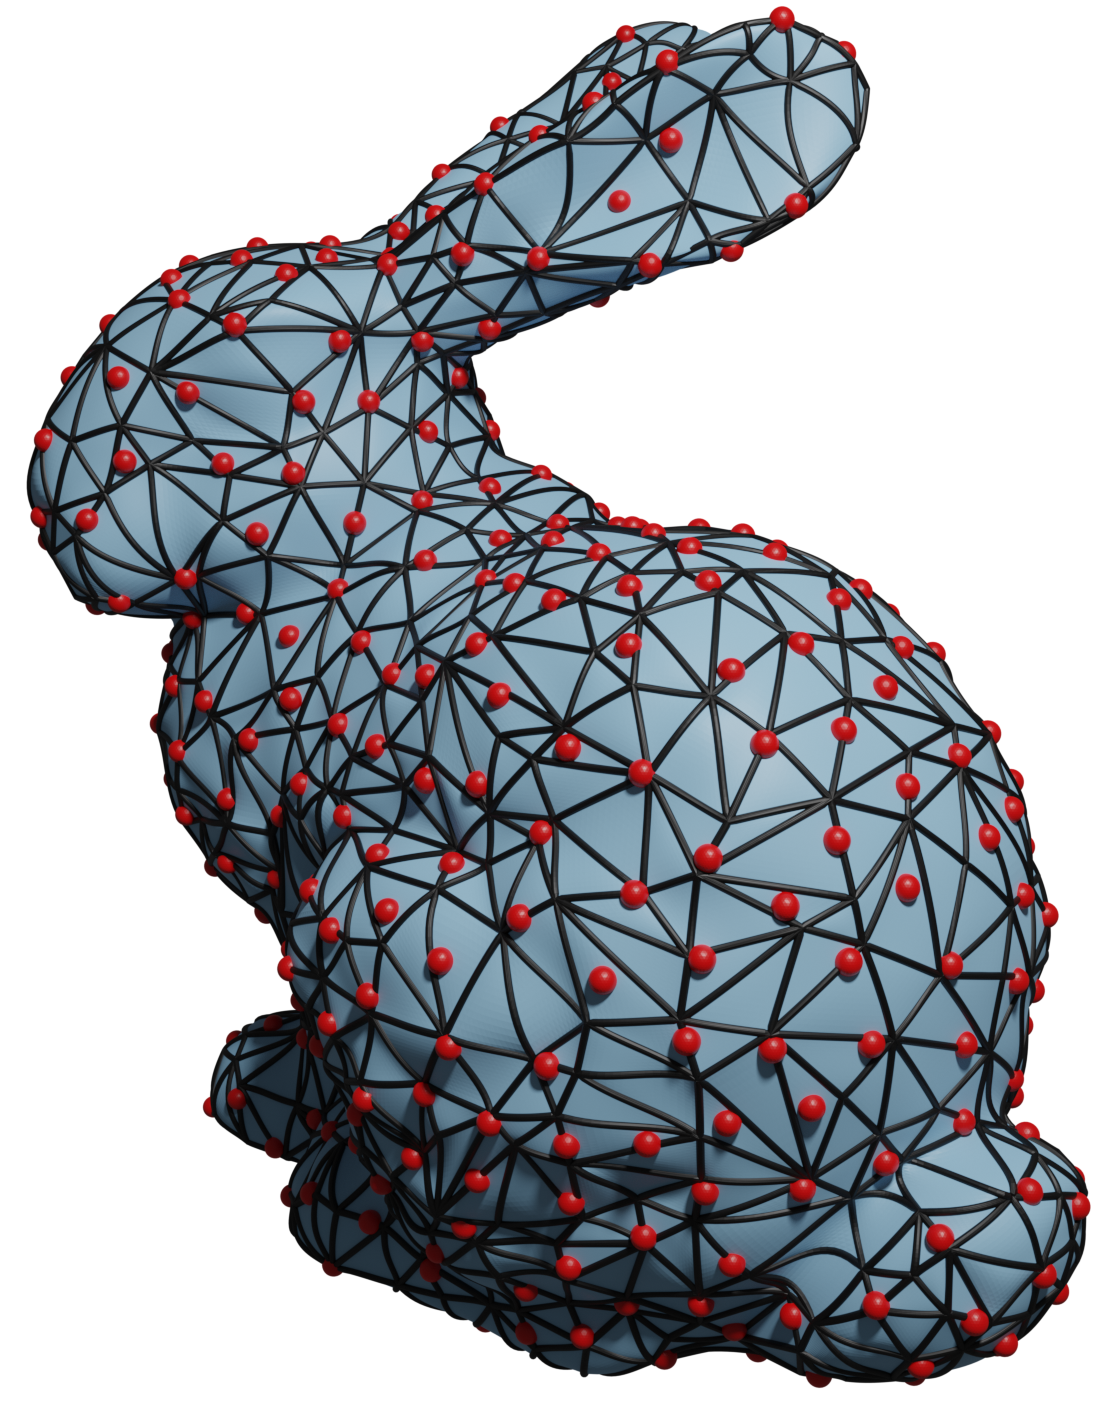
\includegraphics[width=0.23\linewidth]{curve_meshing_in_shell_tex/figs/bunny/0003}\hfill
    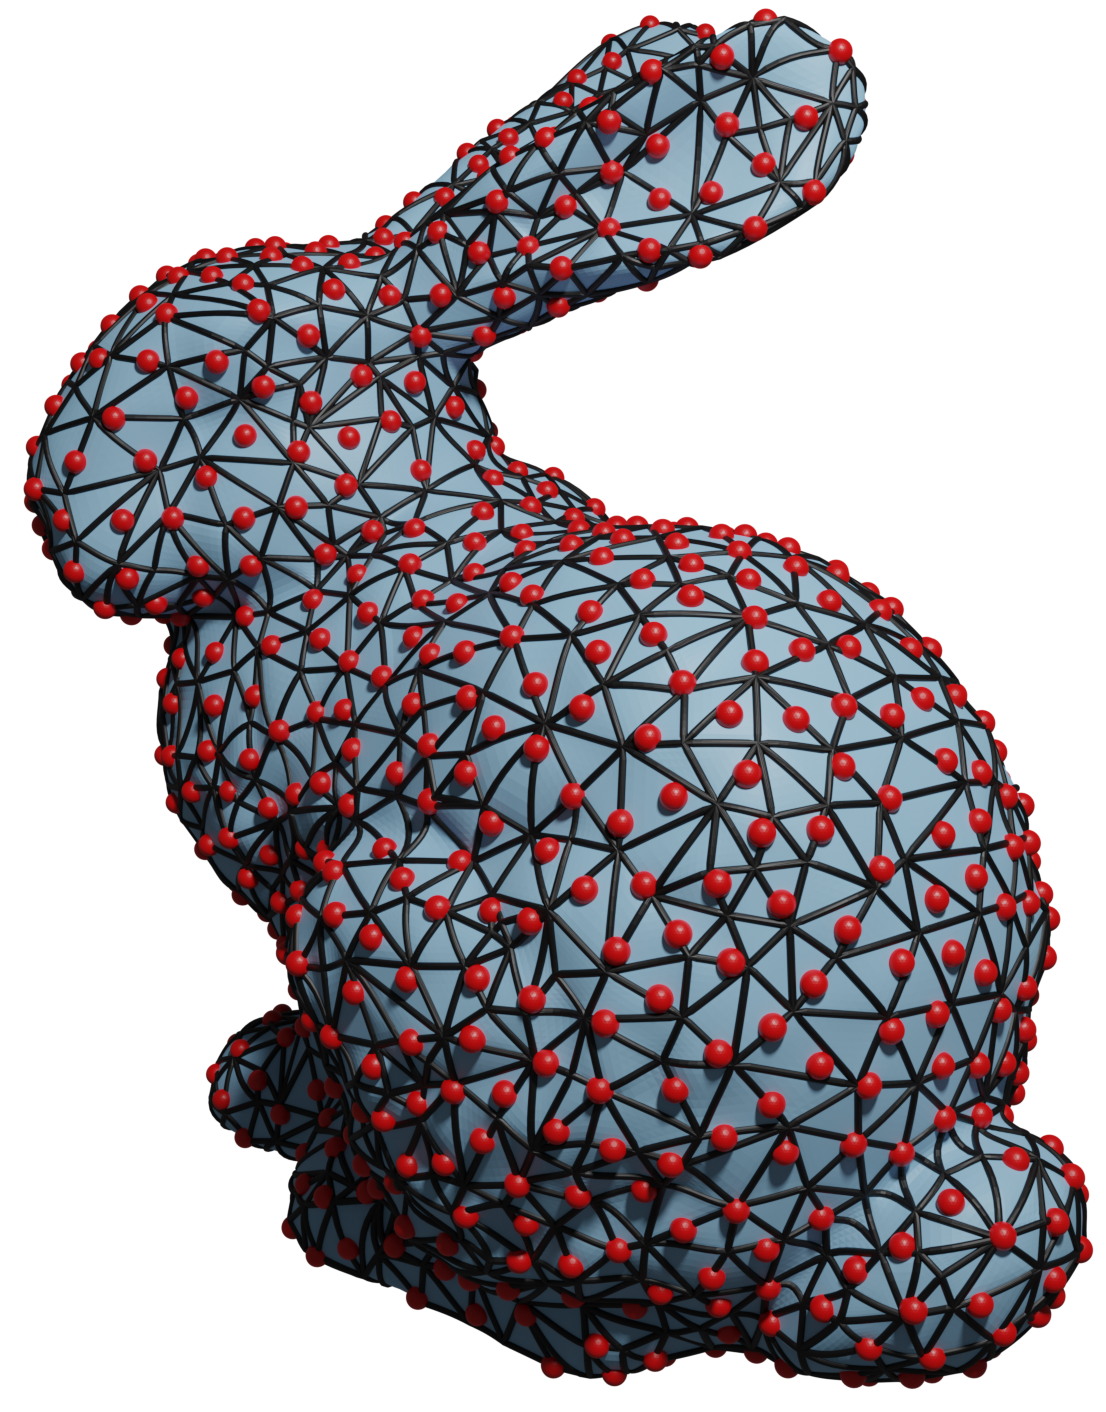
\includegraphics[width=0.23\linewidth]{curve_meshing_in_shell_tex/figs/bunny/0002}\par
    \parbox{.23\linewidth}{\centering 0 points.}\hfill
    \parbox{.23\linewidth}{\centering 200 points.}\hfill
    \parbox{.23\linewidth}{\centering 500 points.}\hfill
    \parbox{.23\linewidth}{\centering 1000 points.}
    \caption{Effect of the choice of the set $\P$ on the output.}
    \label{bichon:fig:points-effect}
\end{figure}



We are not assuming anything on $\P$: a sparse set of points will generate a mesh less faithful to the input geometry, while a dense sampling computed for instance with Poisson disk sampling~\cite{bowers2010parallel} will prevent the surface from deviating too much (Figure~\ref{bichon:fig:points-effect}).


Our algorithm guarantees that the tetrahedralization is positive and that $\partial\T^k$ does not have self-intersections. 
It also aims at coarsening {$\T^k$} as much as possible while striving to obtain a good geometric quality. 
To reliable fit $\partial \T^k$ to $\M$ we require a bijective map
\[
\phi^k \colon \M \to \partial \T^k
\]
from the input $\M$ to the surface of $\T^k$ (Figure~\ref{bichon:fig:input-output} right). Our algorithm also generates this map and exposes it as an output for additional uses, such as attribute transfer. Note that, since we build upon the shell construction in~\ref{chp:shell}, we also {guarantee} $\partial\T^k$ is homeomorphic and topology-preserving with respect to $\M$ (Figure~\ref{bichon:fig:intersection}).


\begin{figure}
    \centering
    % \includegraphics{}
    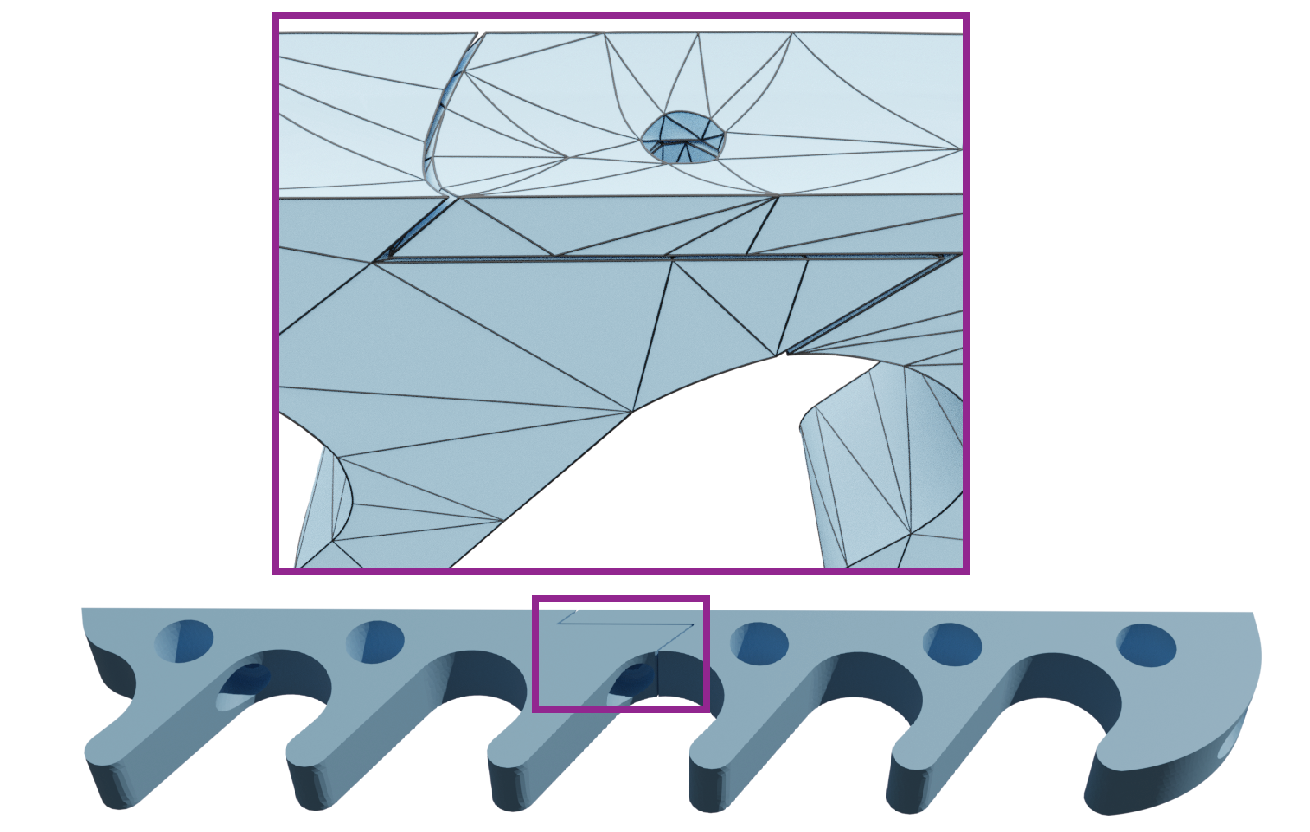
\includegraphics[width=0.9\linewidth]{curve_meshing_in_shell_tex/figs/intersection-free.pdf}\hfill
    \caption{Our algorithm maintains {free of} intersection even on challenging models, without the need of setting adaptive threshold.}
    \label{bichon:fig:intersection}
\end{figure}


%For each edge provided in the feature annotation list, 
%there exists one curved edge in the output mesh, 
%where the marked edge is in bijective correspondence to a segment in the curved edge.


To simplify the explanation{,} we use the bar $\overline{\phantom{M}}$ to represent quantities on the \emph{straight} linear shell, the tilde $\widetilde{\phantom{M}}$ for the \emph{curved} shell, and hat $\hat{\phantom{M}}$ for the reference elements (e.g., $\overline P$ is the prism on {the} straight coarse shell, $\widetilde P$ is the curved prism, and $\hat P$ is the prism on the reference configuration).


\begin{definition}\label{def:curved-mesh}
We call a curved mesh $\T^k$ and its mapping $\phi^k$ to $\M$ \emph{valid} if it satisfies the following conditions:
\begin{enumerate}
    \item $\phi^k$ is bijective;
    \item the distance between any $p\in\P$ and $\partial\T^k$ is less than $\varepsilon$;
    \item $\T^k$ is positive (i.e., every geometric map $g^\tau$ has positive Jacobian's determinant).
\end{enumerate}
\end{definition}

\paragraph{Overview.} 
Our algorithm starts by creating a valid mesh (i.e., it satisfies~\ref{def:curved-mesh}), then it performs local operations (Appendix~\ref{app:local-ops}) to improve $\T^k$ (i.e., coarsen it and improve its quality) while ensuring all the conditions remain valid with respect to local modification. 
To achieve this goal, our algorithm uses two stages: (1) curved shell generation and (2) tetrahedral mesh generation and optimization.

\begin{figure}
    \centering
    % \includegraphics[width=\linewidth]{curve_meshing_in_shell_tex/figs/pipeline1}
    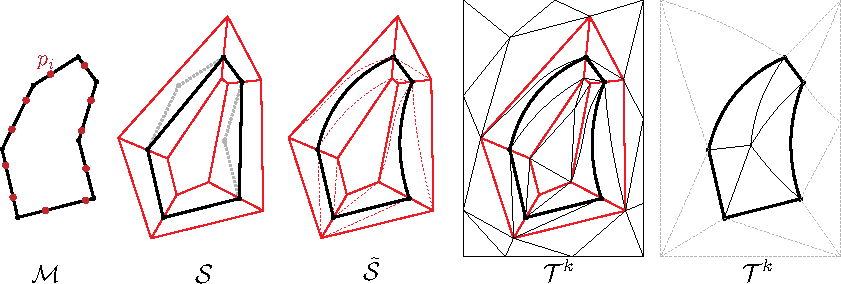
\includegraphics[width=\linewidth]{curve_meshing_in_shell_tex/figs/illustrations/pipeline.pdf}
    \caption{Overview of curved mesh generation pipeline.}
    \label{bichon:fig:pipeline}
\end{figure}

\paragraph{Stage 1: Curved Shell Construction.}
In the first stage (Section~\ref{cumin:sec:high-order}) we extend the shell construction of~\ref{chp:shell} by combining the shell projection $\Pi$ with {a} high-order mapping 
\[
\psi^k \colon \prS \to \PS.
\]
We start form the \emph{valid} shell $\PS$ constructed from the input mesh $\M$ (i.e., $\M$ is a section $\PS$). We call $\PS$ a \emph{\ps{}} and call the prismatic projection $\Pi$. Together with the construction of $\PS$, we build an order $k$ \emph{curved prismatic shell} $\prS$ that defines a curved layer around $\M$ and a \emph{bijective} map $\psi^k$ between $\prS$ and $\PS$ (Figure~\ref{bichon:fig:pipeline}, first three figures) that ensures that the distance between $\M$ and $\partial\T^k$ is smaller than $\varepsilon$ (Section~\ref{cumin:sec:distance}). That is, $\phi^k(p) < \varepsilon$ for any $p\in\P$. (Note that we do not require $\M$ to be a section of $\prS$.)

To facilitate the volumetric meshing in the next stage (Section~\ref{cumin:sec:tets}), we restrict the top and bottom surface of $\prS$ to be linear (independently from the order of $\psi^k$). The final output of this first stage is a high-order volumetric shell,
a bijective mapping $\phi^k = \Pi \circ \psi^k$,
and a \emph{positive} tetrahedralization of $\prS$ with flat boundary. In other words, the tetrahedralization of $\prS$ satisfies~\ref{def:curved-mesh}.

\paragraph{Stage 2: Tetrahedral Mesh Generation.}
In the second stage (Section~\ref{cumin:sec:tets}) we use boundary-conforming tetrahedralization to connect the top and bottom surface of $\prS$ with a background tetrahedral mesh, thus generating a \emph{positive} order $k$ tetrahedralization $\T^k$ of a bounding box around the input, which we can further optimize with local operations to improve its quality  (Figure~\ref{bichon:fig:pipeline}, last two figures). % Note that this pipeline  decouples the surface generation and feature preservation problem from the conforming volumetric tassellation, enabling us to tackle these two challenges independently.


To ensure that our first condition is satisfied{,} we define the mapping $\phi^k$ as a composition of several mappings{,} which we ensure are bijective. 
For the second condition, we initialize our construction with $\phi^k$ {as} the identity, {and} thus, the distance at the sample points is zero. 
After every operation, we recompute the distance and ``undo'' the operation if the distance becomes larger than $\varepsilon$. To ensure that the last condition holds, we rely on checking if all prisms (linear and curved) have positive geometric mapping, which {ensures} that they can be tetrahedralized with a positive tetrahedralization. 
Ensuring the condition while coarsening $\M$ {allows} us to generate a coarse \emph{curved} tetrahedral mesh $\T^k$ and the \emph{bijective} map $\phi^k$ to the input mesh $\M$.


\subsection{High-order Shells}\label{cumin:sec:high-order}
To simplify the explanation, we first focus on the case where $\varepsilon = \infty$, that is, we aim at generating {an} as-coarse-as-possible curved mesh. Note that, the trivial solution (i.e., a single tetrahedron) is not necessary a valid $\T^k$ since it would be impossible to build the bijective mapping $\phi^k$.

The output of~\ref{chp:shell} is a coarse shell $\PS$ with {a} piecewise linear middle surface. To curve it, we construct a shell $\prS$ and the bijective map $\psi^k$ while constructing $\PS$. 
The shell $\prS$ is constructed warping every prism $\widetilde P$ of $\prS$ with $\psi^k$. Since we define $\phi^k$ as  $\Pi \circ \psi^k$, and $\Pi$ satisfies the first two conditions~\ref{def:curved-mesh}, we only need to ensure that $\psi^k$ is bijective, for $\phi^k$ to be bijective.  We define the mapping $\psi^k = \overline\omega\circ(\widetilde\omega^k)^{-1}$ {through} two {cross-parametrization} maps from the reference prism $\hat P$: 
\[
% \text{(1) } 
\overline\omega \colon \hat P \to \overline P, \qquad
% \text{(2) } 
\widetilde\omega^k \colon \hat P \to \widetilde P.
\]

Both mappings $\overline\omega$ and $\widetilde\omega^k$ are defined as the tensor product between the base triangular mapping (high-order for $\widetilde\omega^k$) and pillar's {barycentric} heights. That is, for a prism $\widetilde P$
\[
\widetilde\omega^k (\hat u,\hat v, \hat h) = 
% \sum_{i=1}^3 
\sum_{j=1}^n c_j^P L_j(\hat u,\hat v) \big((1-\hat u - \hat v)  h_1^{\widetilde P}+ \hat u h_2^{\widetilde P} + \hat v  h_3^{\widetilde P}\big)\hat h,
\]
where $\hat u,\hat v,\hat h$ are the barycentric coordinates in the reference prism, $c_j$ the control points of a triangle, $h_i^{\widetilde P}$ the three pillars heights, and $L_j$ a triangle polynomial basis.
By ensuring that $\psi^k$ is bijective, we guarantee that any curved tetrahedralization of a prism $\widetilde P$ will be a valid tetrahedralization of $\prS$.

We note that to decouple the following tetrahedral mesh generation and the curved shell generation, we ensure that $\widetilde\omega^k$ maps the top and bottom face of the curved prism $\widetilde P$ to a linear triangle.

After each local operation, we generate samples $\hat s_i, i=1,\dots,m$ on the parametric base of the prism $\hat P$ and use $\Pi^{-1}\circ \overline\omega$ to map $\hat s_i$ back to $\M$ and $\widetilde \omega^k$ to map them to $\partial\T$. Using the mapped point we solve
\[
\min_{c_i} \sum_{i=1}^m \|
(\Pi^{-1}\circ \overline\omega)(\hat s_i) - 
\widetilde \omega[c_i]^k(\hat s_i)
\|_2^2,
\]
where $c_i$ are the control points of $\widetilde\omega^k$. As $\widetilde \omega[c_i]^k(\hat s_i)$ is a linear function of $c_i$. This is a quadratic optimization problem.
The control points of the top and bottom surface are fixed to ensure that $\widetilde\omega^k$ maintains the two surfaces as linear. We validate the bijectivity of
$\widetilde\omega^k$ by checking positivity of the determinant~\cite{johnen2013geometrical} and that the top and bottom surfaces are intersection free. The intersection is simplified in our case since fast and exact algorithms\cite{guigue2003fast} are available since the top and bottom surfaces stay linear.



\begin{figure}
    \centering\small
    % \includegraphics{}
    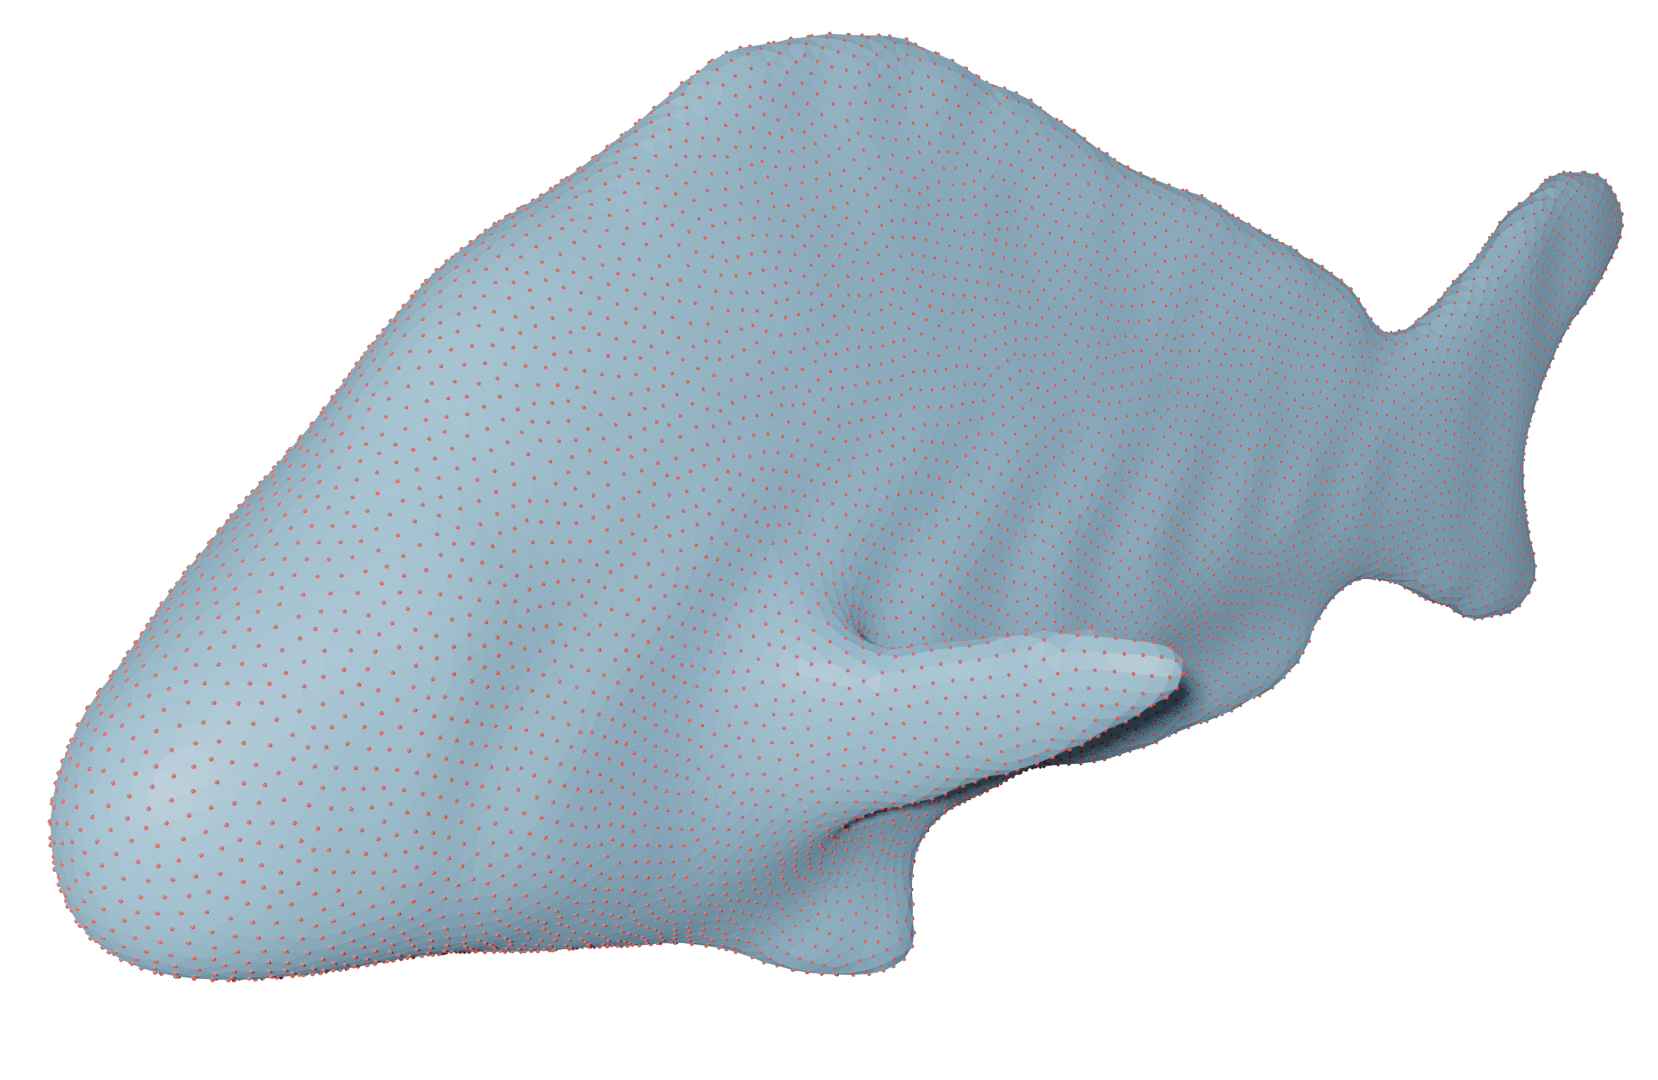
\includegraphics[width=.23\linewidth]{curve_meshing_in_shell_tex/figs/fish/fish002}
    \hfill
    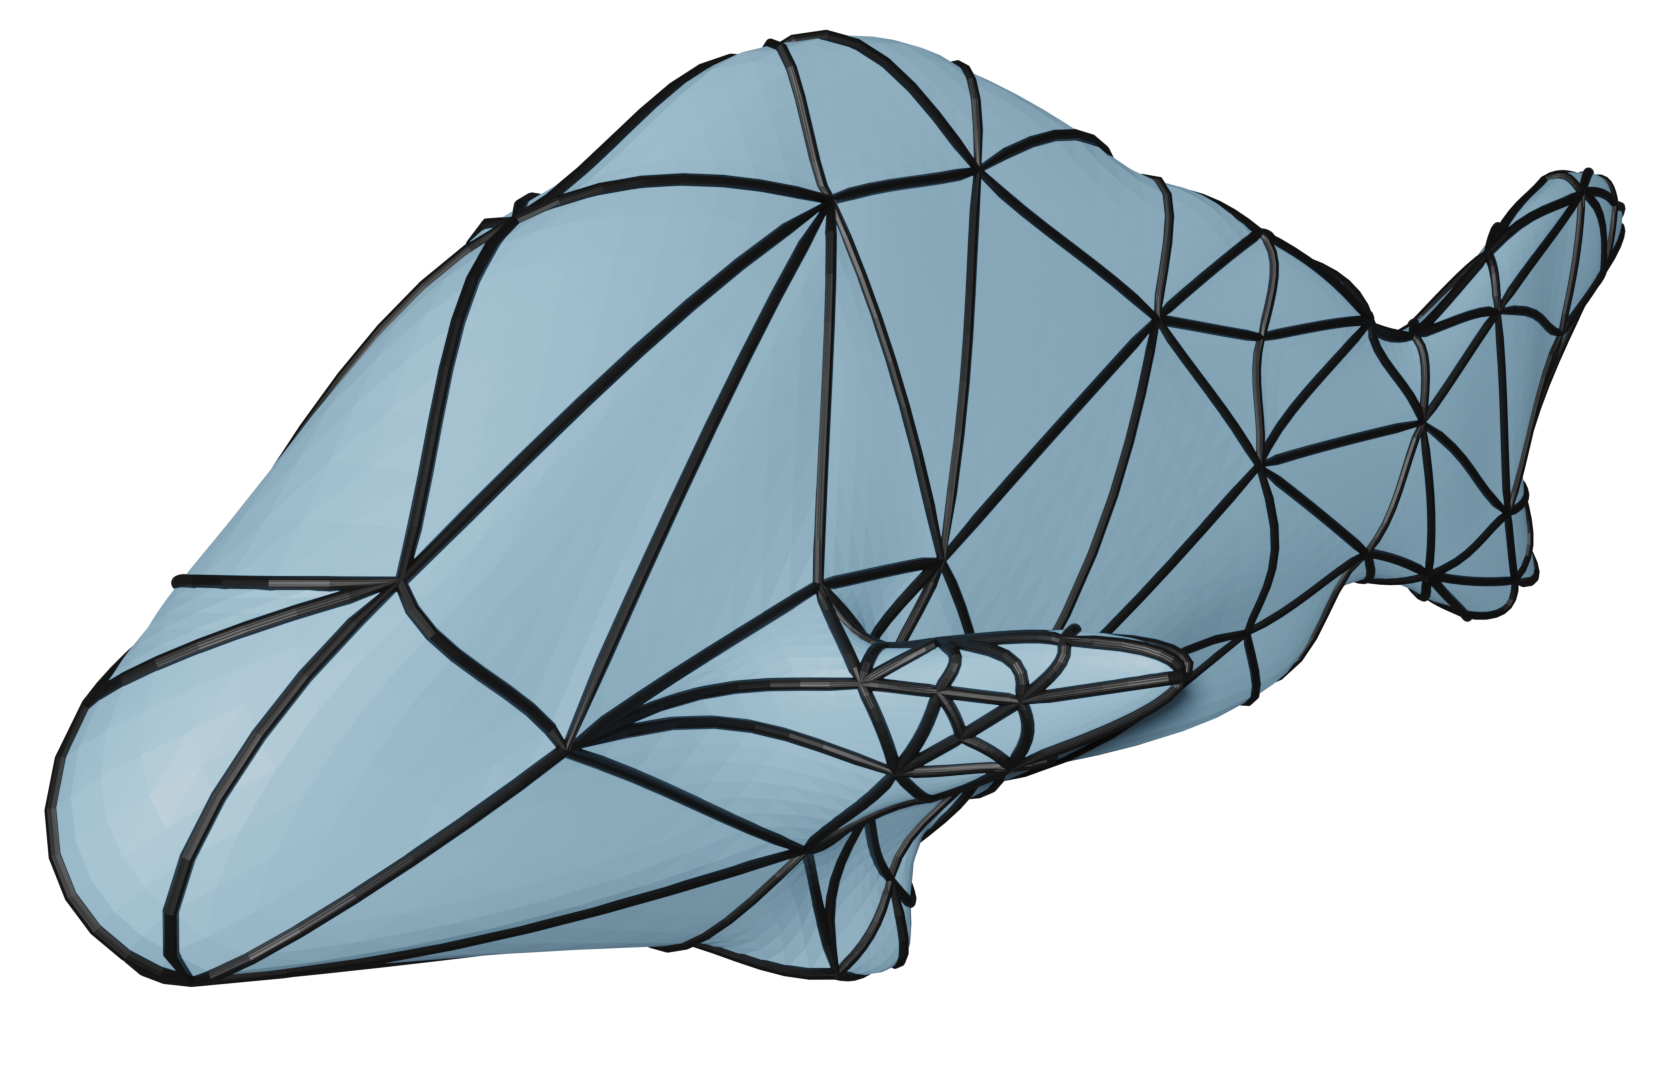
\includegraphics[width=.23\linewidth]{curve_meshing_in_shell_tex/figs/fish/0003}\hfill
    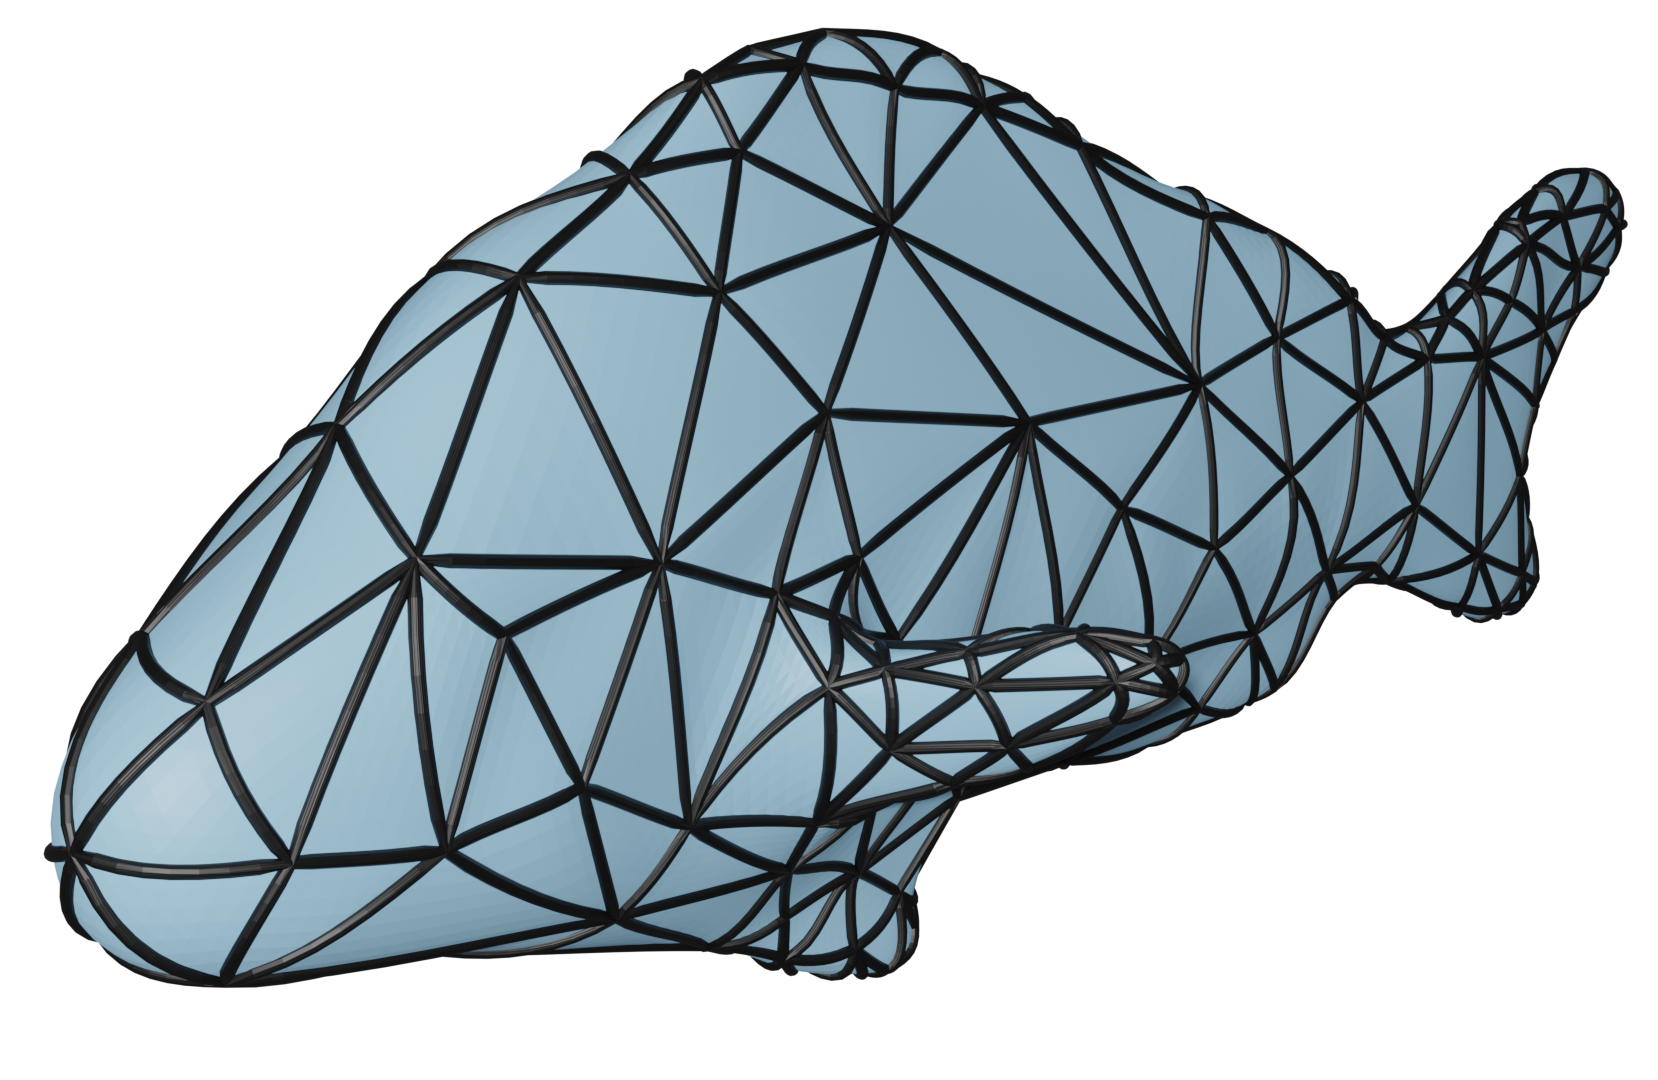
\includegraphics[width=.23\linewidth]{curve_meshing_in_shell_tex/figs/fish/0001}\hfill
    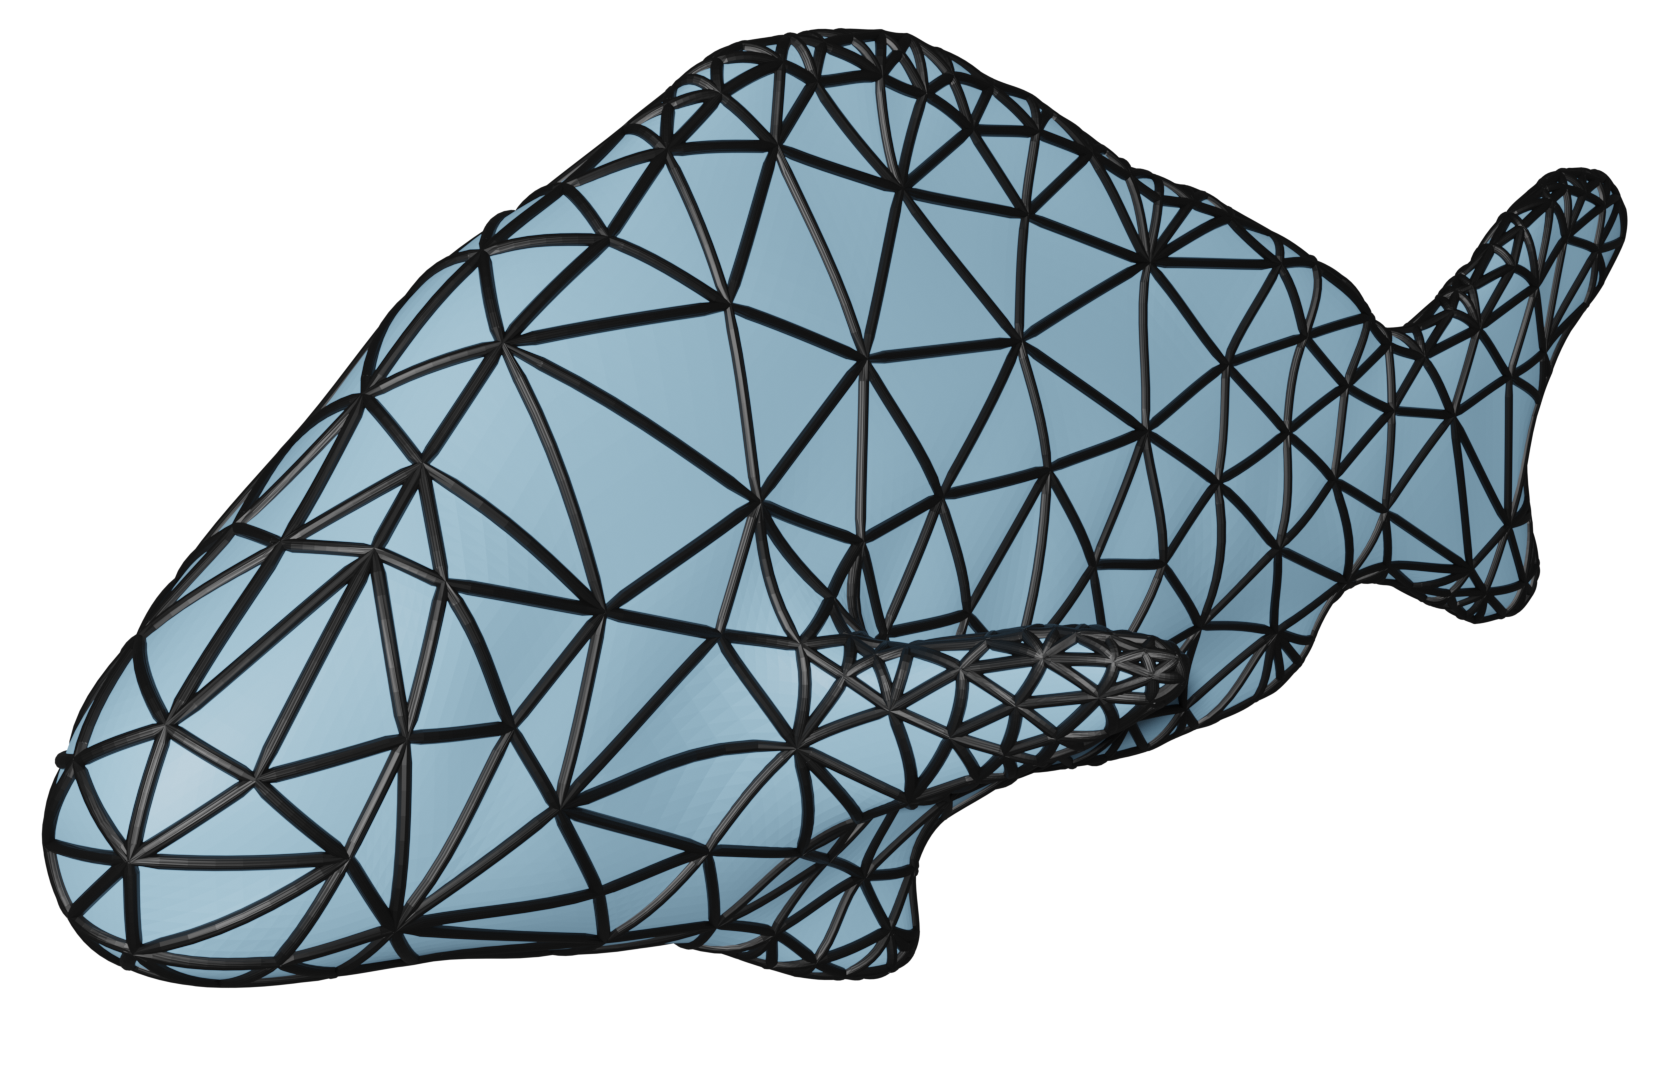
\includegraphics[width=.23\linewidth]{curve_meshing_in_shell_tex/figs/fish/0004}\par
    \parbox{.23\linewidth}{\centering Input}\hfill
    \parbox{.23\linewidth}{\centering $\varepsilon =5\times 10^{-3}$}\hfill
    \parbox{.23\linewidth}{\centering $\varepsilon =  10^{-3}$}\hfill
    \parbox{.23\linewidth}{\centering $\varepsilon = 5\times 10^{-4}$}
    \caption{A model simplified with different distances.}
    \label{bichon:fig:distance}
\end{figure}

\subsection{Distance Bound}\label{cumin:sec:distance}

In the previous section, we explained how to generate a curved shell $\prS$ that satisfies~\ref{def:curved-mesh}. To ensure that the middle surface of $\prS$ has a controlled distance from the points in $\P$, we interleave a distance check in the construction of $\widetilde\omega^k$ after each local operation. Formally, after every local operation we use the mapping $\phi^k$ to map every point $p_i\in\P$ to $\widetilde p_i = \phi^k(p_i)$ a point on the coarse curved middle surface of $\prS$ and, if $\|p_i-\widetilde p_i\| \geq \varepsilon$ we reject the operation. The initial shell is trivially a valid initialization as $\phi^k$ is identity and thus, the distance is zero. Note that, $\widetilde p_i$ is not necessarily the closest point to $p_i$ on $\partial\T$, thus $\|p_i-\widetilde p_i\|$ is an upper bound on the actual pointwise distance. Figure~\ref{bichon:fig:distance} shows the effect of the distance bound on the surface; a small distance will lead to a denser mesh with more details, while a {large} one will allow for more coarsening.



%%%%%%%%%%%%%%%%%%%%%%%%%%%%%%%%%%%%%%%%%%%%%%%%%%%%%%%%%%%%%%%%
%%%%%%%%%%%%%%%%%%%%%%%%%%%%%%%%%%%%%%%%%%%%%%%%%%%%%%%%%%%%%%%%
\subsection{Tetrahedral Meshing}\label{cumin:sec:tets}

The outcome of the previous stage is a curved tetrahedralization of $\prS$ that closely approximates $\M$ with linear (``flat'') boundaries. We now consider the problem of filling its interior (and optionally its exterior) with a tetrahedral mesh, a problem known as  \emph{conforming boundary preserving} tetrahedralization. 

%After the linear tetrahedralization, we have a valid (according to Definition~\ref{def:curved-mesh}) output which we further improve by performing local operations on the curved mesh.

\begin{figure}
    \centering
    % \includegraphics[width=.39\linewidth]{curve_meshing_in_shell_tex/figs/tet12}\hfill
    % \includegraphics[width=.39\linewidth]{curve_meshing_in_shell_tex/figs/tet34}\hfill
    % \includegraphics[width=.19\linewidth]{curve_meshing_in_shell_tex/figs/tet5}
    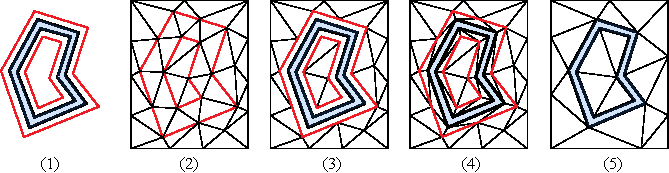
\includegraphics[width=\linewidth]{curve_meshing_in_shell_tex/figs/illustrations/conforming-overview.pdf}
    \caption{Two dimensional overview of the five steps of our boundary preserving tetrahedral meshing algorithm.}
    \label{bichon:fig:conforming-overview}
\end{figure}

Several solution exists for this problem (Section~\ref{cumin:sec:rel:linear}) and the most common implementation is TetGen~\cite{si2015tetgen}. Most algorithms refine the boundary, which allows {deriving} bounds on the quality of the tetrahedral mesh. However, in our setting, this is problematic, as any change will have to be propagated to the curved shell. To avoid coupling the volumetric meshing problem with the curved shell coarsening, while technically possible it is very challenging to implement robustly, we opt for using a tetrahedral meshing algorithm that preserves the boundary exactly. Not many algorithms support this additional constraint, the only one with a public implementation is the widely used TetGen algorithm. However, we discovered that, when this option is used, it suffers from robustness issues, which we detail in Appendix \ref{app:tetgen}.
%
To solve this problem in our specific setting, we propose in the following five step algorithm (Figure~\ref{bichon:fig:conforming-overview}) taking advantage of the availability of a shell, based on the  TetWild~\cite{hu2018tetrahedral} algorithm. %\DP{Can we avoid it?} We refer to Appendix~\ref{app:tetwild} for a brief overview of the TetWild algorithm.
% Without loss of generality we focus the explanation to the bottom surface, as for the top surface it is equivalent.

\paragraph{Step 1.}
To generate a boundary preserving linear mesh, we first exploit the shell to extrude the bottom surface $B$ (and top $T$) {further} by a positive (potentially small) constant $\delta$ such that the newly extruded bottom surface $B_e$ (and top $T_e$) does not self-intersect. The space between $B$ and $B_e$ (and between $T$ and $T_e$) consists of prisms {divided} into positive tetrahedra. 

\paragraph{Step 2.}
Then we insert $B_e$ and $T_e$ in a background mesh $\B$ generated following TetWild algorithm (\cite[Section 3.1]{hu2018tetrahedral}), that is, we use the triangle of $B_e$ and $T_e$ as the input triangle meshes for the first stage of the TetWild algorithm, which inserts them into a background mesh $\B$, so that
each input triangle is a union of faces of refinement of $\B$.


We interrupt the algorithm after the  binary space partitioning (BSP) subdivision (and before the TetWild mesh optimization \cite[Section 3.2]{hu2018tetrahedral})
to obtain a positive tetrahedral mesh in rational coordinates with a surface with the same geometry of $B_e$ and $T_e$, but possibly different connectivity as TetWild might refine it during the BSP stage.

\paragraph{Step 3.}
Our original goal was to compute a mesh conforming to $B$ and $T$, but we could not do it directly with TetWild as they might be refined. We now replace the mesh generated by TetWild between $B_e$ and $T_e$ with another one conforming to $B$ and $T$. To achieve this, we delete all tetrahedra between $B_e$ and $T_e$, and insert the surfaces $B$ and $T$, which will ``float'' in the empty space between $B_e$ and $T_e$. We now want to fill the space between $B$ and $B_e$ with positive tetrahedra conforming to the surfaces $B$ and $T$. 

\paragraph{Step 4.}
Every prism $P$, made by a bottom triangle $B^T$ and a bottom extruded triangle $B_e^T$ and its corresponding bottom extruded refined triangle $B_e'^T \in \B$, can be tetrahedralized without refining $B$: That is, we first decompose the prism $B^T, B_e^T$ in tetrahedra (always possible by construction), then refine every tetrahedron touching $B_e'^T$. By repeating the same operation on the space between $T$ and $T_e$ we will have a positive linear boundary conforming tetrahedral mesh of $B$ and $T$. 

\paragraph{Step 5.}
The tetrahedra generated in the previous step will have rational coordinates and will also likely have low quality. To round the coordinates to floating-point representation and to improve their quality, we use the mesh optimization stage of TetWild, with the minor variant of keeping the vertices and edges on $B$ and $T$ frozen. Note that the vertices in $B$ and $T$ are already roundable to floating-point representation, as they were part of the input.


\paragraph{Curved Tetrahedral Mesh Optimization}
After generating the conforming linear tetrahedral mesh. we stitch it with the tetrahedralized $\prS$ to obtain a valid output mesh $\T^k$ {(Definition~\ref{def:curved-mesh}).} However, its quality might be low, in particular in the curved region, as $\prS$ can be thin with large triangles. To improve the quality of  $\T^k$ we adapt the local operation of a linear pipeline to our curved settings. We propose three local operations: smoothing, collapse, and flip. 
Since the surface of $\T^k$ is already coarse {and} of high quality, {as} part of the definition of $\phi^k$, we prevent any local operation from changing it. We validate every local operation (i.e., check the positivity of $\T^k$) using the convex-hull property~\cite{johnen2013geometrical} and reject the operation if it is violated.
Our local operations are prototypical, and we leave as future work a more comprehensive study of curved mesh optimization.
 
\paragraph{Smoothing.} As for the linear case, we compute the total energy of a vertex $v$ by summing up the energies of the tetrahedra adjacent to it, which we compute on 56 regularly sampled points. 
We then perform gradient descent {for} all high-order nodes in the one-ring neighborhood of $v$. That is, we collect all edge nodes, face nodes, and cell nodes of the one-ring neighborhood of $v$. Differently {from} the linear case, the optimization is expensive since the nodes neighborhood typically contains hundreds of nodes.

\paragraph{Collapse and Swap}
The collapse and swap are the same as in a linear mesh, and we place the high-order nodes of the newly created face on the linear flat face.